% !TEX program = xelatex
% DeepPersona 코드 학습교재 — 모듈 05: 깊이우선 값 채우기 (generate_profile.py, Step 5)
\documentclass[aspectratio=169,10pt]{beamer}
\usetheme{metropolis}
\metroset{block=fill,numbering=fraction,progressbar=frametitle,sectionpage=progressbar}
\usepackage{kotex}\usepackage{fontspec}
\setmainhangulfont{Apple SD Gothic Neo}\setsanshangulfont{Apple SD Gothic Neo}\setmonofont{D2Coding}
\usepackage{booktabs}\usepackage{array}\usepackage{graphicx}\usepackage{amssymb}\usepackage{amsmath}
\usepackage{tikz}\usetikzlibrary{arrows.meta,positioning,fit,backgrounds,calc}
\usepackage{listings}

\definecolor{accent}{HTML}{0E7C7B}\definecolor{navy}{HTML}{004191}\definecolor{orange}{HTML}{F97316}
\definecolor{ink}{HTML}{20242A}\definecolor{muted}{HTML}{5A6472}\definecolor{blockbg}{HTML}{EDF1F6}
\definecolor{codebg}{HTML}{E7ECF3}\definecolor{kw}{HTML}{0D6E6E}\definecolor{str}{HTML}{A8410F}\definecolor{com}{HTML}{5A6472}
\definecolor{bad}{HTML}{B0402F}
\setbeamercolor{progress bar}{fg=accent}\setbeamercolor{title separator}{fg=accent}\setbeamercolor{frametitle}{bg=accent}
\setbeamercolor{alerted text}{fg=orange}\setbeamercolor{block title}{bg=blockbg,fg=ink}\setbeamercolor{block body}{bg=blockbg!55,fg=ink}

\newcommand{\lead}[1]{\vspace*{0.6em}{\setlength{\fboxsep}{9pt}\noindent\colorbox{accent!12}{\parbox{\dimexpr\textwidth-2\fboxsep\relax}{\textcolor{accent}{\textbf{한눈에}}\hspace{0.6em}#1}}}\par\vspace{1.15em}}
\newcommand{\intu}[1]{\vspace*{0.2em}{\setlength{\fboxsep}{7pt}\noindent\colorbox{navy!8}{\parbox{\dimexpr\textwidth-2\fboxsep\relax}{\textcolor{navy}{\textbf{쉽게 말하면}}\hspace{0.6em}#1}}}\par\vspace{0.5em}}
\newcommand{\srcnote}[1]{\vspace{0.35em}\par{\footnotesize\color{navy}$\blacktriangleright$~#1}}
\newcommand{\pc}[1]{\tikz[baseline=(pcb.base)]{\node[fill=codebg,rounded corners=2pt,inner xsep=3pt,inner ysep=1pt,outer sep=0pt,anchor=base] (pcb) {\ttfamily\footnotesize #1};}}
\lstdefinestyle{py}{basicstyle=\ttfamily\scriptsize,backgroundcolor=\color{codebg!55},keywordstyle=\color{kw}\bfseries,stringstyle=\color{str},commentstyle=\color{com}\itshape,language=Python,showstringspaces=false,breaklines=true,frame=leftline,framerule=1.4pt,rulecolor=\color{accent},xleftmargin=12pt,aboveskip=3pt,belowskip=2pt,tabsize=2}

\title{DeepPersona 코드 학습교재}
\subtitle{모듈 05 — 깊이우선 값 채우기: \texttt{generate\_profile.py} (Step 5)}
\author{학습 정리 덱 (Claude와 함께)}
\institute{원저: Wang et al., \textit{DeepPersona} (arXiv:2511.07338) · 논문 \S3.2 "Progressive LLM filling"}
\date{\today}

\begin{document}
\maketitle

\begin{frame}{이 모듈의 목표}
  \lead{고른 슬롯에 LLM이 \alert{값}을 채운다 — 카테고리를 순서대로, 앞의 결과를 맥락으로 받아 \emph{일관되게}.}
  \begin{columns}[T]
    \begin{column}{0.5\textwidth}
      \small\textbf{얻는 것}
      \begin{itemize}
        \item \alert{depth-first} 순차 생성의 뜻
        \item 카테고리별 \alert{조건부 프롬프트}
        \item 값 생성 코드(1 카테고리=1 LLM 호출)
        \item \pc{Summary} 서사 생성
        \item \alert{카테고리 drop 버그}(19$\to$6)
      \end{itemize}
    \end{column}
    \begin{column}{0.5\textwidth}
      \small\textbf{핵심 통찰}
      \begin{itemize}
        \item 각 카테고리는 \emph{앞의 모든 카테고리}를 reference로 받음 $\to$ 전역 일관성
        \item 값은 \alert{$\le$100자}로 캡 $\to$ 얕은 narrative
        \item 6개만 명시 처리 $\to$ \alert{13개 조용히 누락}
      \end{itemize}
    \end{column}
  \end{columns}
  \srcnote{이 모듈이 식 (2)의 \emph{generator} $\Pr_\theta(v_i\mid a_i,S,P_{<i})$에 해당.}
\end{frame}

\begin{frame}{순서}\tableofcontents\end{frame}

% ============================================================
\section{1. Progressive filling}
% ============================================================
\begin{frame}{깊이우선 — \alert{앞을 보고 다음을 쓴다}}
  \intu{이력서를 위에서부터 채우듯, 인구통계 $\to$ 직업 $\to$ 가치관 순으로, 매번 \emph{지금까지 쓴 것}을 보며 다음 칸을 채운다.}
  \begin{columns}[T]
    \begin{column}{0.5\textwidth}
      \textbf{논문 "Progressive LLM filling"}
      \begin{itemize}\small
        \item selector가 슬롯 $a_i$를 고르면, generator $\theta$가 값 $v_i$를 채움
        \item $v_i$는 \emph{지금까지의 프로필} $P_{<i}$에 \alert{조건부}
        \item 그래서 뒤 값이 앞 값과 안 어긋남(전역 일관성)
      \end{itemize}
    \end{column}
    \begin{column}{0.5\textwidth}
      \begin{block}{독립 생성이면?}
        각 슬롯을 따로 채우면 "35세 은퇴 CEO인데 대학생" 같은 모순 발생.
      \end{block}
      \begin{block}{조건부 생성이면}
        직업을 쓸 때 이미 만든 나이·인구통계를 보고 씀 $\to$ 앞뒤 일치.
      \end{block}
    \end{column}
  \end{columns}
  \lead{진입점 \pc{generate\_single\_profile(attribute\_count=200)} — 시드$\to$선택$\to$값채우기$\to$Summary를 한 번에.}
\end{frame}

% ============================================================
\section{2. 카테고리 순차 생성}
% ============================================================
\begin{frame}{7개 카테고리를 \alert{순서대로}, 앞을 참조하며}
  \intu{카테고리를 하나씩 채우되, 각 단계 프롬프트에 앞서 만든 카테고리를 통째로 "참고자료"로 넣는다.}
  \begin{center}
  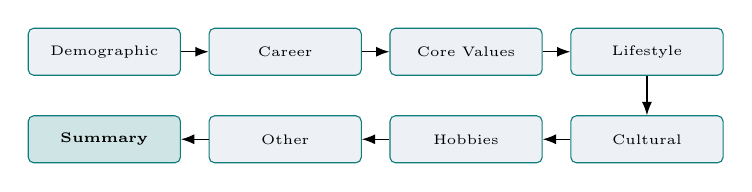
\begin{tikzpicture}[font=\tiny,>=Latex,
      b/.style={draw=accent,fill=blockbg,rounded corners=2pt,align=center,inner sep=2.5pt,text width=5.0em,minimum height=1.7em}]
    \node[b] (d) {Demographic};
    \node[b,right=0.35cm of d] (c) {Career};
    \node[b,right=0.35cm of c] (v) {Core Values};
    \node[b,right=0.35cm of v] (l) {Lifestyle};
    \node[b,below=0.5cm of l] (cu) {Cultural};
    \node[b,left=0.35cm of cu] (h) {Hobbies};
    \node[b,left=0.35cm of h] (o) {Other};
    \node[b,fill=accent!20,left=0.35cm of o] (s) {\textbf{Summary}};
    \draw[->](d)--(c);\draw[->](c)--(v);\draw[->](v)--(l);\draw[->](l)--(cu);
    \draw[->](cu)--(h);\draw[->](h)--(o);\draw[->](o)--(s);
  \end{tikzpicture}
  \end{center}
  \begin{itemize}\footnotesize
    \item 각 화살표 = "앞 카테고리 JSON을 \pc{for reference}로 프롬프트에 주입".
    \item 예: Career 프롬프트엔 이미 만든 Demographic이, Hobbies엔 Demo+Career+Values+Lifestyle+Cultural 전부가 들어감.
  \end{itemize}
  \lead{이 "누적 참조"가 곧 $P_{<i}$ 조건부 — 코드로 구현된 \alert{depth-first breadth}.}
\end{frame}

\begin{frame}[fragile]{조건부 프롬프트 — 앞 결과를 통째로 넣는다}
  {\scriptsize 파일: \pc{generate\_profile.py} · Career 단계 입력 구성(발췌)}
\begin{lstlisting}[style=py,numbers=none,basicstyle=\ttfamily\tiny]
career_input = (
  "Base Information (for reference):\n" + json.dumps(base_info,...) + "\n\n"
  "Life Story (for reference):\n" + str(life_story) + "\n\n"
  "Demographic Information (for reference):\n"          # <- 앞서 만든 것!
    + json.dumps(profile.get("Demographic Information", {}),...) + "\n\n"
  "Instructions: ... develop the 'Career and Work Identity' ... "
  "evident or reasonably inferred from base_info, life_story, Demographic ...")
\end{lstlisting}
  \begin{itemize}\footnotesize
    \item \textbf{누적}: 뒤 카테고리일수록 \pc{profile.get("...")}로 앞 카테고리를 더 많이 참조.
    \item \textbf{"inferred from"}: 새 사실을 지어내지 말고 \emph{앞 정보에서 추론}하라고 지시 $\to$ 일관성.
    \item \textbf{생성 순서} = \pc{Demographic $\to$ Career $\to$ Core Values $\to$ Lifestyle $\to$ Cultural $\to$ Hobbies $\to$ Other}.
  \end{itemize}
  \srcnote{프롬프트마다 "balance" 류 단어 금지 등 스타일 제약도 포함(반복 표현 억제).}
\end{frame}

\begin{frame}[fragile]{값 생성 — 카테고리 1개 = LLM 호출 1번}
  {\scriptsize 파일: \pc{generate\_profile.py} · \texttt{generate\_category\_attributes()}}
\begin{lstlisting}[style=py,numbers=none,basicstyle=\ttfamily\tiny]
def collect_leaf_paths(obj, current_path):        # 카테고리 아래 모든 leaf 수집
    for key, value in obj.items():
        path = f"{current_path}.{key}" if current_path else key
        if isinstance(value, dict) and not value: leaf_paths.append(path)  # 빈{}=leaf
        elif isinstance(value, dict): collect_leaf_paths(value, path)
system_prompt = "Format as JSON: key=attribute path, value=... (<=100 characters)."
user_prompt = custom_prompt + "\n".join(f"- {p}" for p in leaf_paths)
response = get_completion(messages)               # 한 번에 전체 leaf 값 생성
generated_values = json.loads(cleaned_response)   # {path: value, ...}
\end{lstlisting}
  \begin{itemize}\footnotesize
    \item \textbf{leaf 수집}: 카테고리 하위의 빈 \pc{\{\}}(=슬롯)를 경로로 모음.
    \item \textbf{1회 호출}: 그 카테고리의 \emph{모든 슬롯을 한 번의 LLM 호출로} 채움(호출 수 절약).
    \item \textbf{값 캡 \alert{$\le$100자}}: 각 값이 짧게 강제됨 $\to$ narrative가 얕아지는 원인.
    \item \textbf{파싱}: 마크다운 \pc{```json} 펜스를 벗기고 \pc{json.loads} $\to$ \pc{\{경로:값\}}.
  \end{itemize}
  \srcnote{이후 \pc{parts=path.split('.')}로 \{경로:값\}을 다시 중첩 dict로 복원해 프로필에 넣음.}
\end{frame}

\begin{frame}[fragile]{Summary — 전체를 \alert{서사}로 엮는다}
  {\scriptsize 파일: \pc{generate\_profile.py} · \texttt{generate\_final\_summary()}}
\begin{lstlisting}[style=py,numbers=none,basicstyle=\ttfamily\tiny]
profile_for_summary = profile.copy()
for key in ['base_info','personal_story','interests','Occupations']:
    profile_for_summary.pop(key, None)            # 원재료 제거(중복 방지)
final_summary_text = generate_final_summary(profile_for_summary, base_info)
profile["Summary"] = final_summary_text           # 100~400 단어 1인칭 서사
\end{lstlisting}
  \begin{itemize}\footnotesize
    \item \textbf{입력}: 완성된 구조적 프로필 전체(원재료 키는 제거).
    \item \textbf{출력}: 100$\sim$400단어의 통합 narrative(부족하면 경고, 초과하면 400단어로 절삭).
    \item \textbf{역할}: 논문의 $\mathrm{Narr}(P)$ — 구조적 속성을 사람이 읽는 이야기로. (Fig 2 우하단 "Summary")
  \end{itemize}
  \lead{산출물 = \alert{구조적 속성(200개) + 서사 Summary}. 이게 한 페르소나 $P$.}
\end{frame}

% ============================================================
\section{3. 카테고리 drop 버그}
% ============================================================
\begin{frame}[fragile]{버그: \alert{6개만} 처리, 13개 조용히 누락}
  {\scriptsize 파일: \pc{generate\_profile.py} · 각 단계가 \emph{정확한 이름}으로만 꺼냄}
\begin{lstlisting}[style=py,numbers=none,basicstyle=\ttfamily\tiny]
demographic_template = selected_paths.get("Demographic Information")
career_template      = selected_paths.get("Career and Work Identity")
core_template        = selected_paths.get("Core Values, Beliefs, and Philosophy")
lifestyle_template   = selected_paths.get("Lifestyle and Daily Routine")
cultural_template    = selected_paths.get("Cultural and Social Context")
hobbies_template     = selected_paths.get("Hobbies, Interests, and Lifestyle")
other_template       = selected_paths.get("Other Attributes")   # 데이터에 없음 -> None!
\end{lstlisting}
  \begin{itemize}\footnotesize
    \item \textbf{원인 1}: 모듈 02의 top-level이 \alert{19개}(중복 variant). 그런데 여기선 \emph{정확한 6개 문자열}만 \pc{.get()}.
    \item \textbf{원인 2}: 나머지 13개(예: "Core Values \emph{and} Beliefs", "Lifestyle and Habits", "Education and Learning" \dots)를 잡을 \pc{"Other Attributes"} 키가 selected\_paths에 \alert{없음} $\to$ \pc{None} $\to$ skip.
    \item \textbf{결과}: 19개 중 \alert{6개(32\%)}만 값이 채워지고 13개는 흔적 없이 사라짐.
  \end{itemize}
  \srcnote{selected\_paths는 카테고리별 dict인데, 중복 variant를 "Other Attributes"로 묶는 로직이 없다.}
\end{frame}

\begin{frame}{버그의 영향 \& 수정 방향}
  \intu{그래서 광고된 "1MB narrative"가 실제론 27KB에 그친다 — 슬롯은 골라졌는데 값 채우기에서 대부분 버려져서다.}
  \begin{columns}[T]
    \begin{column}{0.5\textwidth}
      \textbf{실측(count=350, study.md \S13)}
      \begin{center}\footnotesize
      \renewcommand{\arraystretch}{1.15}
      \begin{tabular}{@{}lcc@{}}\toprule
        & 실제 & README 주장 \\\midrule
        프로필 크기 & \alert{27 KB} & $\sim$1 MB \\
        채워진 속성 & 200 & 200+ \\
        처리 카테고리 & \alert{6/19} & (전부 가정) \\
        \bottomrule
      \end{tabular}
      \end{center}
    \end{column}
    \begin{column}{0.5\textwidth}
      \textbf{수정 방향}
      \begin{itemize}\footnotesize
        \item selected\_paths의 \alert{모든 top-level 키를 동적 순회}(하드코딩 6개 대신)
        \item 모듈 02의 \pc{merge\_tree.py}로 중복 variant를 12개로 \alert{정규화}
        \item 값 캡 100자 완화 $\to$ narrative 길이↑
      \end{itemize}
    \end{column}
  \end{columns}
  \lead{다음 bottleneck은 임베딩이 아니라 \alert{여기(카테고리 매핑)}다 — 재현 시 반드시 인지.}
\end{frame}

\begin{frame}{이 모듈 요약}
  \begin{columns}[T]
    \begin{column}{0.5\textwidth}
      \textbf{꼭 기억할 것}
      \begin{itemize}
        \item depth-first = 앞 카테고리를 \alert{참조}하며 채움
        \item 카테고리 1개 = LLM 호출 \alert{1번}
        \item 값 \alert{$\le$100자}, Summary는 100$\sim$400단어
        \item \alert{6/19}만 처리(카테고리 drop 버그)
        \item 병목은 임베딩이 아니라 \alert{매핑}
      \end{itemize}
    \end{column}
    \begin{column}{0.5\textwidth}
      \textbf{함수 지도}
      \begin{itemize}\footnotesize
        \item \pc{generate\_single\_profile} (진입점)
        \item \pc{generate\_category\_attributes} (값 생성)
        \item \pc{collect\_leaf\_paths} (슬롯 수집)
        \item \pc{generate\_final\_summary} (서사)
      \end{itemize}
    \end{column}
  \end{columns}
  \lead{다음 \pc{06\_run\_reproduce}: 실제로 돌려 페르소나를 \alert{재현}하고 pkl을 고친다.}
\end{frame}

\begin{frame}[standout]
  모듈 05 끝\\[0.4em]
  {\normalsize 다음: \texttt{06\_run\_reproduce} — 실행·재현·스크립트}
\end{frame}

\end{document}
